\documentclass[a4paper,12pt]{article}
\usepackage[utf8]{inputenc}
\usepackage{graphicx}
\usepackage{subcaption}
\usepackage{chngcntr}
\counterwithin{figure}{section}
\usepackage{authblk}
\usepackage{titling}
\setlength{\droptitle}{-10em}   % This eliminates the space on top of title
\usepackage[font=scriptsize]{caption}
\usepackage{float}
\usepackage{siunitx}

%opening
\title{Complex Systems And Networks\\Homwork 2}
\author{Akhil Devarashetti\\Jenna Sawaf}
\begin{document}
  \maketitle

  \section{Schelling's Segregation Model}
  \subsection{System Description}
  We ran the simulation for 10 trails (30 trails was taking more than 12 hours which is too long) with 15 epochs each, with a 50x50 grid and 90\% of the cells are filled with agents i.e. 2250 agents in total. We ran 4 relocation policies simultaneously where initial random distribution of agents is the same for all 4 simulations. The minimum number of surrounding agents of same type to make an agent happy (k) is set to 4 because it yielded satisfactory results while experimenting. The maximum number of random checks in Policy 1 is (q) 100.

  \subsection{Comparing policy 1 and policy 2}
  For the Policy 2, we ran the simulation with the suggested parameters of n = [5, 10, 20] and p = [3, 5] and two additional cases of (n, p) = [(25, 3), (5, 7)], a total of 8 cases. The number of happy agents over each epoch for all trails and all cases is plotted in the Figure \ref{fig:1.1}. Each point at an epoch is the average value at that epoch over all trails.

  \begin{figure}[ht]
    \centering
    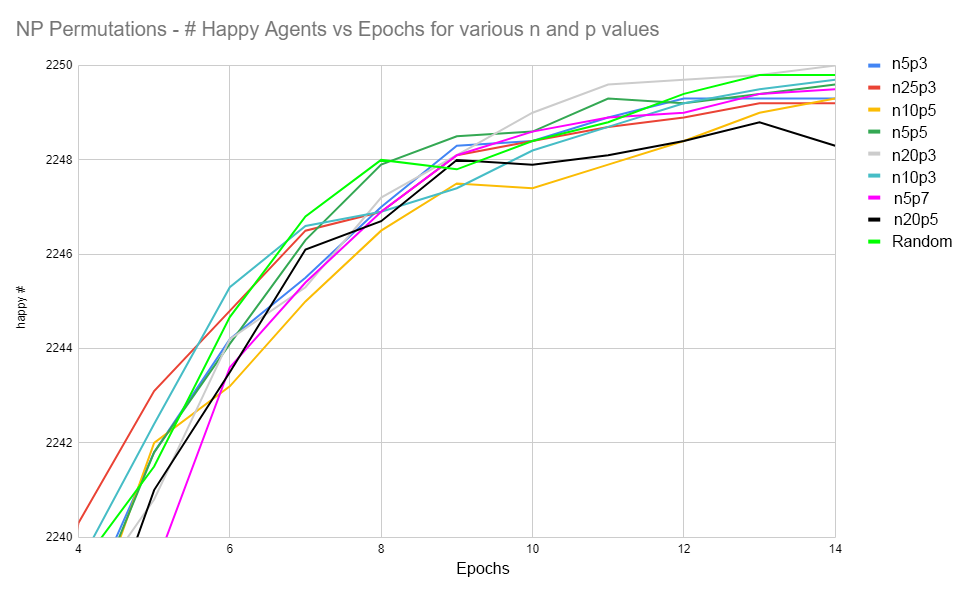
\includegraphics[width=0.9\linewidth]{socialPermutations.PNG}
    \caption{Number of happy agents vs epochs for various n and p values}
    \label{fig:1.1}
  \end{figure}

  Theoretically, the (n, p) pair that can check more number of cells for happiness would have a higher probability of performing better. For example, for the pair (5, 3), the number of cells checked for happiness is 5x3x3 = 45 cells, assuming that these cells are not overlapping, and for the pair (20, 5), the number of cells checked is 20x5x5 = 500. So intuitively, we know that (20, 5) pair will yield better results despite taking longer to run each time step. We call this number n*p*p as the global scope.

  However, upon looking at the results, it looks like all the cases yield a very similar performance. On a closer look, we can see that the pair (25, 3) with a global scope of 500 cells performed worst, followed by (10, 5) with 250 cell global scope. The pair (5, 3) with a global scope of 45 cells turned out to be an average performer. A sweet spot of about 200 cells in the global scope (by (20, 3) and (25, 3) pairs) gave the best results.
  It is not evident that any one of either n or p had an influence on the results independently. Having a greater n alone did not give better results. The results correlate better with the global scope i.e. with both n and p.
  One possible explanation for these results would be that as we increase the global scope, the performance increases until the global scope reaches a sweet spot of 200 cells. This is understandable as the number of cells checked increases, the probability of finding cells that are happy increases. Beyond 200, the performance drops because with more number of cells in the global scope being distributed widely in the grid, the probability of forming a close group of agents decreases.

  Based on the observations, I fixed the values of n and p as 25 and 3 respectively. Wen we compare the plots for Policy 1 and Policy 2, we see that the Policy 1 starts off better than Policy 2. This is because in the beginning of the simulation, the friends might not find as many happy cells as the random 100 cells in the Policy 1 would find. However, as the self-organization progresses, the probability of agent being happy at a random cell decreases because some empty cells are surrounded by more empty cells. With Policy 2 however, the empty cells picked are always nearby other cells. So, although Policy 1 appears to quickly self-organize, Policy 2 seems to perform better in the last few epochs before convergence.


  \newpage
  \subsection{Comparing Policy 3 and Policy 1- Jenna}
  The policy that I created finds an unhappy agent, then from that searches for another unhappy agent of the opposite type and swaps them. The first agent is selected randomly, however the 2nd agent is selected by going through the matrix systematically. The relocation policy does not need any parameters, because for every unhappy agent it finds another one and they are swapped. While coming up with this policy i was inspired by bubble sort. But instead of doing it sequentially, the first agent is selected randomly.

  The second part of the report will be like the first part, but will consist of 1-page sections by each
  group member (with names at the top of each page). Each individual’s page should compare their
  Policy 3 with Policy 1. This is also where you will describe your Policy 3 and explain its logic.
  Since the parameters of Policy 3 will be determined by your choice, you should decide how to
  vary them to explore the space of possibilities in a systematic way. Again, you will plot the time series for Policy 1 and all the cases of your policy, as well as any other figures that help you
  analyze the outcomes. Your text will follow the same guidelines as part 1, but each individual’s
  part should be exactly 1 page including figures and text. Since the figures have to be clear, you
  will have to come up with the best way to summarize your results.

  \newpage
  \subsection{Comparing Policy 4 and Policy 1- Akhil}
  I introduced a relocation policy where the unhappy agent would pick the nearest agent of the same type who has an empty spot around it and relocated to one of those surrounding empty cells randomly. It has no parameters. This relocation policy gives preference to local agents first which I think is more natural because a naive agent will first look into its surroundings and takes its position without looking for a global optimal location. We can observe this behaviour during the simulation. The empty cells appear to slide to a nearby location (which is actually an agent sliding into an empty cell, making it's current location an empty cell). This proves to be a bad solution compared to the policy 1. The easy explanation is that the agent doesn't consider whether the new location would make it happy or not. The only hope for an unhappy agent to become happy is that the probability of getting happier would increase if it relocates to a position around the agent of the same type. It doesn't take the happiness of the closest agent into consideration.

  \begin{figure}[ht]
    \centering
    \begin{subfigure}[b]{0.49\linewidth}
      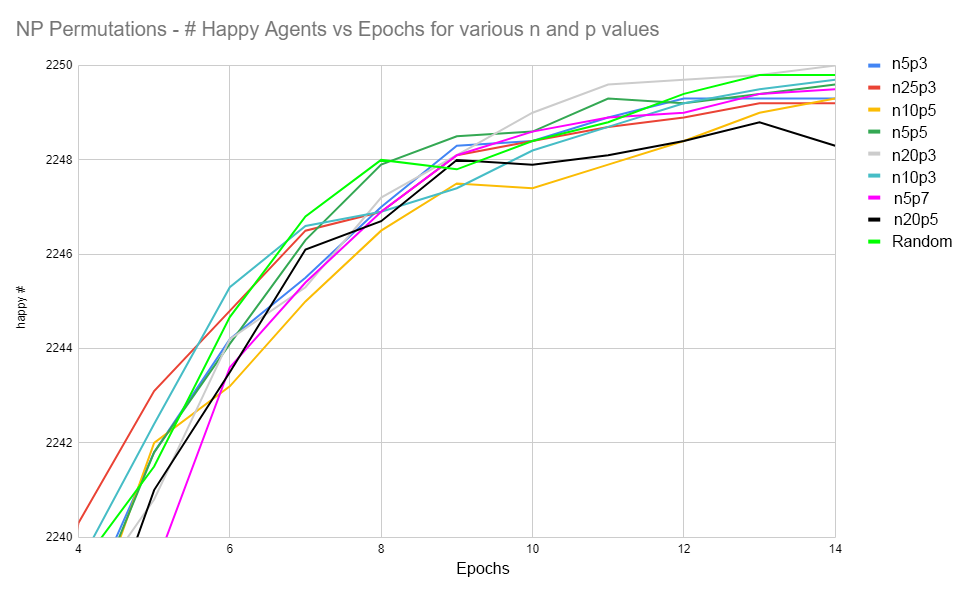
\includegraphics[width=\linewidth]{socialPermutations.PNG}
      \caption{Confusion matrix for train set}
      \label{fig:1.1a}
    \end{subfigure}
    \begin{subfigure}[b]{0.49\linewidth}
      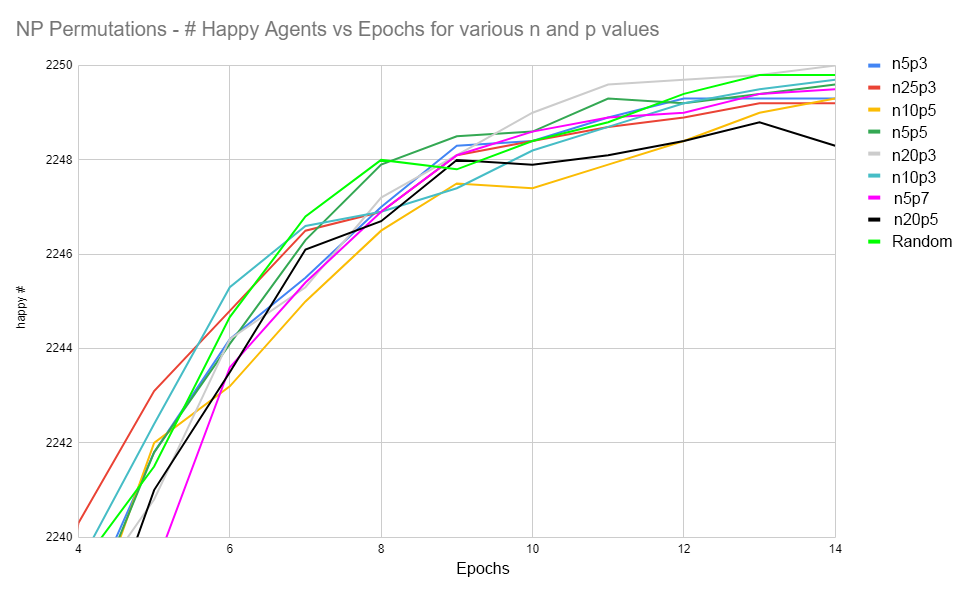
\includegraphics[width=\linewidth]{socialPermutations.PNG}
      \caption{Confusion matrix for test set}
      \label{fig:1.1b}
    \end{subfigure}
    \caption{}
  \end{figure}
  \begin{figure}[ht]
    \centering
    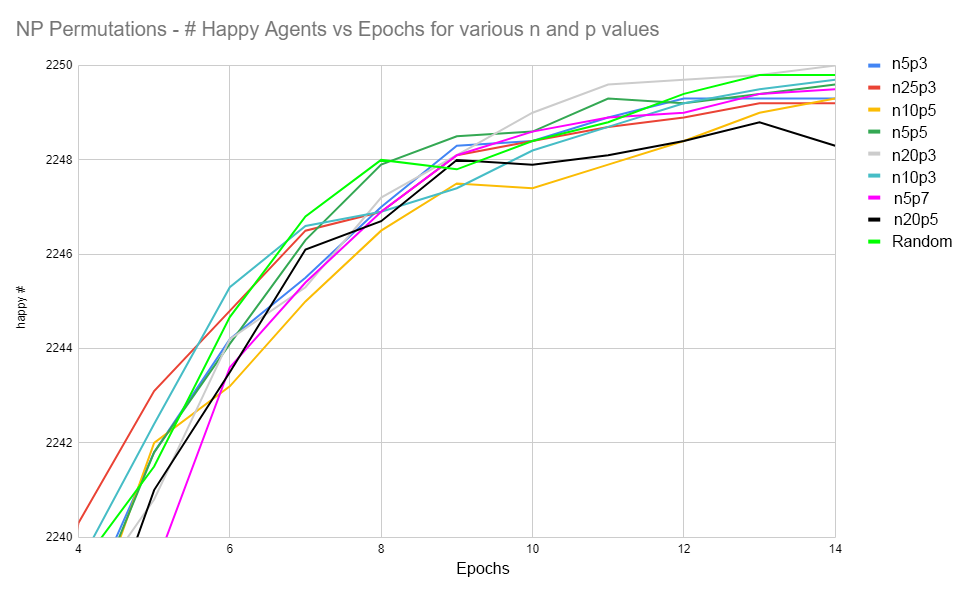
\includegraphics[width=0.5\linewidth]{socialPermutations.PNG}
    \caption{Error in classifying training samples for every 10th epoch}
    \label{fig:1.2}
  \end{figure}

\end{document}
